
\documentclass[10pt,aspectratio=169]{beamer}

\usepackage{algpseudocode, color, colortbl}

\usepackage{wrapfig}

\usetheme{Montpellier}
\usecolortheme{rose}

% page numbers, from
% https://tex.stackexchange.com/questions/137022/how-to-insert-page-number-in-beamer-navigation-symbols
\expandafter\def\expandafter\insertshorttitle\expandafter{%
  \insertshorttitle\hfill%
  \insertframenumber\,/\,\inserttotalframenumber}

\definecolor{Gray}{gray}{0.8}
\newcolumntype{g}{>{\columncolor{Gray}}c}

\newcommand{\stanza}{ \\~\ }

\newcommand{\naive}{na\"{i}ve~}
\newcommand{\Naive}{Na\"{i}ve~}

\title{12. Dynamic Programming for Matrix Chain Multiplication}
\subtitle{CPSC 535}
\author{Kevin A. Wortman}
\institute{ 
\includegraphics[height=2cm]{csuf-logo-cmyk} }
\date{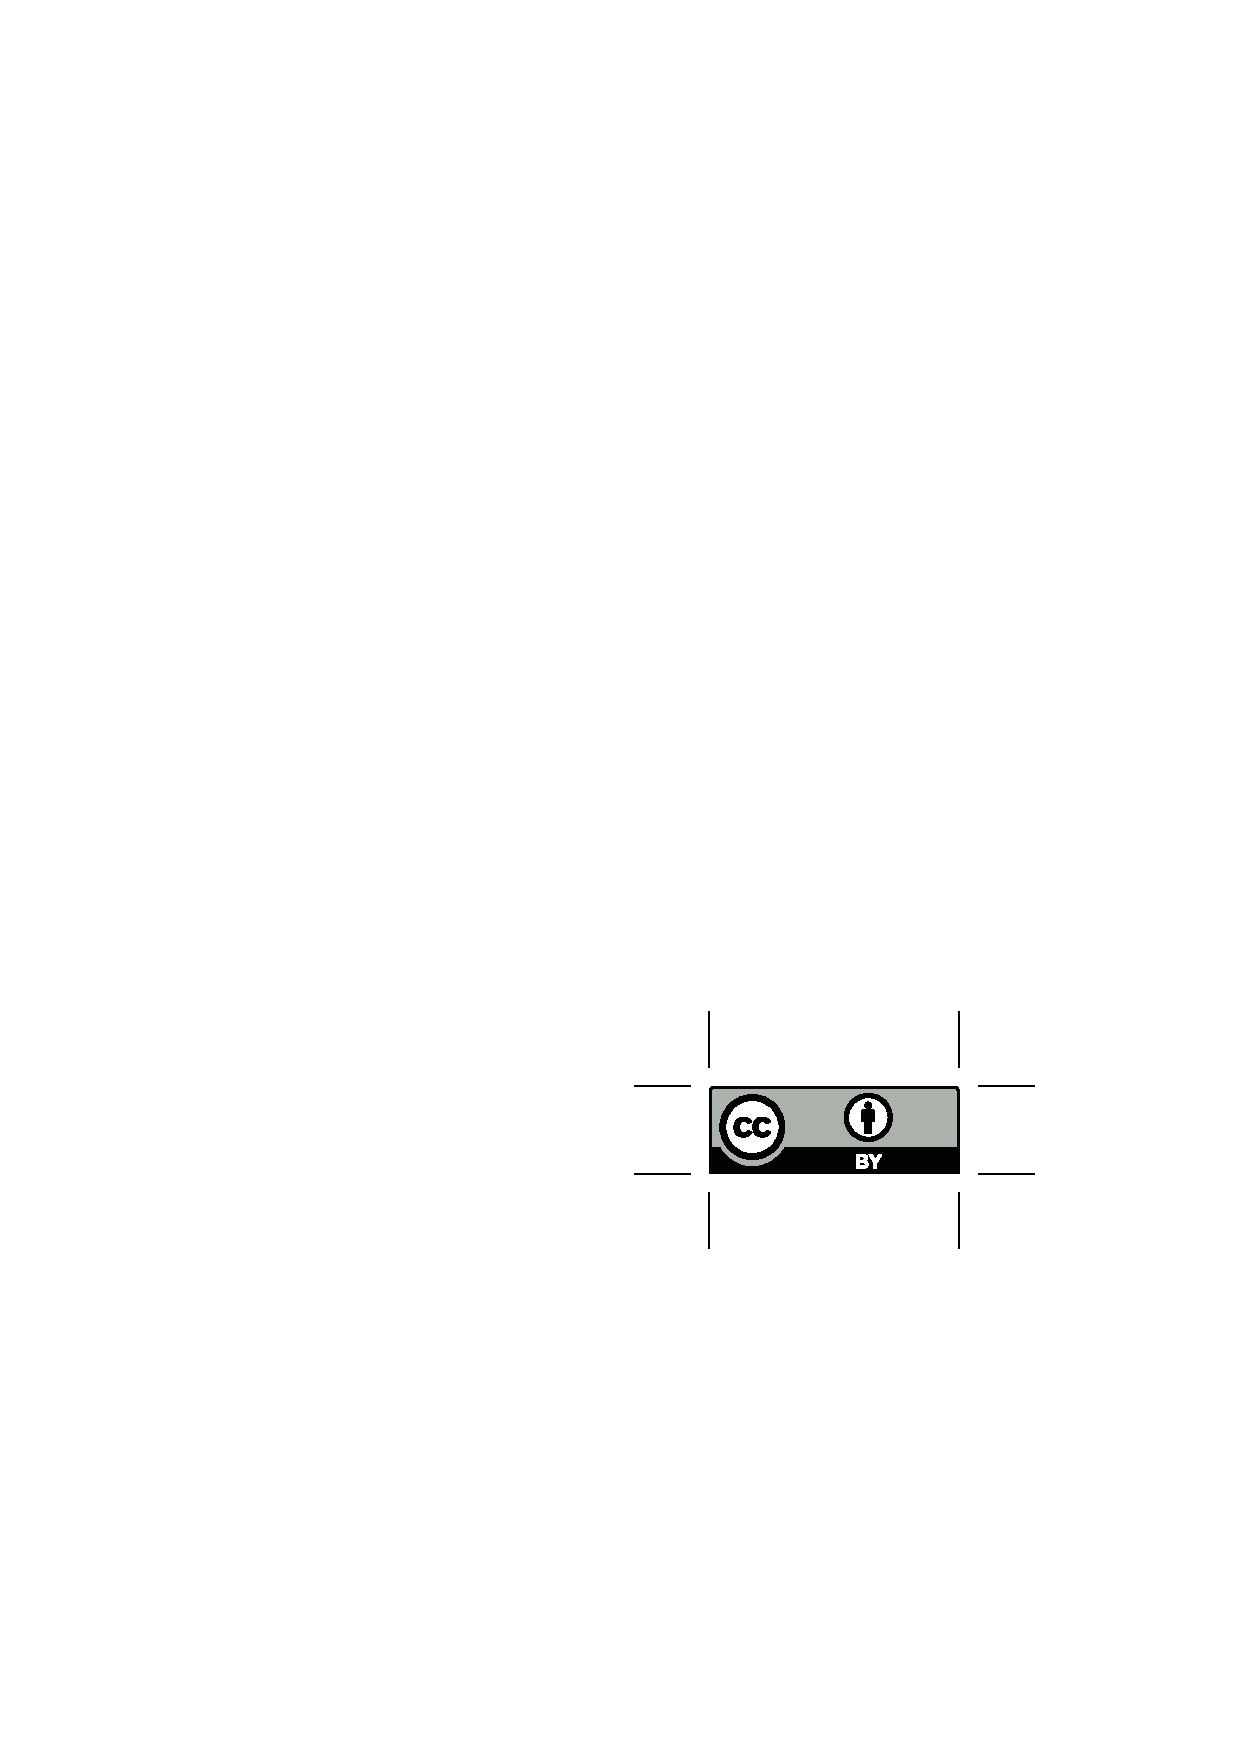
\includegraphics[height=14pt]{by} \\

{\tiny
This work is licensed under a
\href{http://creativecommons.org/licenses/by/4.0/}{Creative Commons Attribution 4.0 International License}.
}}

\begin{document}

\begin{frame}
  \titlepage
\end{frame}

\begin{frame} \frametitle{Big Idea: 2D Table}
\begin{itemize}
  \item \emph{Recall:} dynamic programming
  \begin{itemize}
    \item problem has recursive structure
    \item overlapping subproblems
    \item use table to store solutions, avoid duplicated effort
    \item top-down or bottom-up
  \end{itemize}
  \item so far: \textbf{1D table} -- has one index
  \item now: \textbf{2D table} -- has \emph{two} indices
\end{itemize}
\end{frame}


\begin{frame} \frametitle{Recap: Dynamic Programming Design Process}
  \begin{enumerate}
    \item Identify the problem's \textbf{solution} and \textbf{value}, and note which is our \textbf{goal}.
    \item Derive a \textbf{recurrence} for an optimal value.
    \item Design a divide-and-conquer algorithm that computes an \textbf{optimal value}.
    \item Design a dynamic programming algorithm that computes an \textbf{optimal value}.
    \begin{enumerate}
      \item \textbf{top-down} alternative: add table base case (\textbf{memoization})
      \item \textbf{bottom-up} alternative: rewrite to use bottom-up loops instead of recursion
    \end{enumerate}
    \item (if goal is a solution algo.) Design a dynamic programming algorithm that computes an \textbf{optimal solution}.
  \end{enumerate}
  \end{frame}

\begin{frame} \frametitle{Rod Cutting Step 5}
  \begin{enumerate}
    \setcounter{enumi}{4}
    \item (if goal is a solution algo.) Design a dynamic programming algorithm that computes an \textbf{optimal solution}.
    \stanza
  \end{enumerate}

  
  \emph{rod cutting value problem} \\
  \textbf{input:} an array of non-negative prices $P=\langle p_1, \ldots, p_n \rangle$ \\
  \textbf{output:} the maximum total price that can be achieved by cutting an $n$-inch rod into pieces
  \stanza

  \emph{rod cutting problem} \\
  \textbf{input:} an array of non-negative prices $P=\langle p_1, \ldots, p_n \rangle$ \\
  \textbf{output:} the list of cut-lengths of maximum total price for an $n$-inch rod

\end{frame}

\begin{frame} \frametitle{Recap: Rod Cutting Step 4.b}
  {\small
  \begin{algorithmic}[1]
    \Function{CUT-ROD-BU}{P[1..n]}
    \State Create array $R[0..n]$
    \State $R[0] = 0$
    \For{$j$ from 1 to $n$}
      \State $q=-\infty$
      \For{$i$ from 1 to $j$}
        \State{$q = \max(q, P[i] + R[j-i])$}
      \EndFor
      \State $R[j] = q$
    \EndFor
    \State \Return $R[n]$
    \EndFunction
  \end{algorithmic}
  }
\end{frame}

\begin{frame} \frametitle{Moving from Values to Solutions}
  \begin{itemize}
    \item \textbf{value} version of rod cutting: output is a number (total price)
    \item \textbf{solution} version: output is a list of cuts
    \item Example: for input $n=11,$ output might be $\langle 4, 4, 2, 1 \rangle$
    \item Na\"{i}ve approach: $R[i]$ stores a list of cuts, instead of just a number
  \end{itemize}
\end{frame}

\begin{frame} \frametitle{Rod Cutting Step 5 -- First Draft}
  {\small
  \begin{algorithmic}[1]
    \Function{CUT-ROD-SOLUTION}{P[1..n]}
    \State Create array $R[0..n]$ 
    \State $R[0] = \langle \rangle$ \Comment{empty sequence}
    \For{$j$ from 1 to $n$}
      \State $q= \langle \rangle $
      \For{$i$ from 1 to $j$}
        \State cut-i $= R[j-i] \cup \langle j \rangle$ \Comment{copy of $R[j-i]$ with $j$ appended}
        \If{ TOTAL-PRICE($P,$ cut-i) $>$ TOTAL-PRICE($P, q$) }
          \State $q = $ cut-i
        \EndIf
      \EndFor
      \State $R[j] = q$
    \EndFor
    \State \Return $R[n]$
    \EndFunction
  \end{algorithmic}
  }
\end{frame}


\begin{frame} \frametitle{Rod Cutting Step 5 -- First Draft}
  {\small
  \begin{algorithmic}[1]
    \Function{TOTAL-PRICE}{P[1..n], cuts}
      \State $x = 0$
      \For{$j$ in cuts}
        \State $x = x + P[j]$
      \EndFor
      \State \Return $x$
    \EndFunction
  \end{algorithmic}
  }
\end{frame}

\begin{frame} \frametitle{Analysis}
\begin{itemize}
  \item worst-case length of an $R[j]$ is $\Theta(n)$
    \begin{itemize}
      \item (all 1-cuts)
    \end{itemize}
  \item so TOTAL-PRICE takes $\Theta(n)$ time
  \item creating each cut-i takes $\Theta(n)$ time
  \item CUT-ROD-SOLUTION takes $\Theta(n^3)$ time
  \item \textbf{space} is an issue: CUT-ROD-SOLUTION takes $\Theta(n^2)$ space
\end{itemize}
\end{frame}

\begin{frame} \frametitle{Backtracking}
  \begin{itemize}
    \item algorithm computes optimal value, and \textbf{logs (records) how it made each decision}
    \item after all optimal values have been computed, follow a ``trail'' to create solution object
    \item trail ends at the optimal solution
    \item each log entry says how to go one step backwards
    \item follow them until we get to the start (a base case)
    \item traverses solution in backwards order; reverse it if order matters
    \item backtracking is usually only $\Theta(n)$ time, and $\Theta(n)$ space overhead
  \end{itemize}
\end{frame}

\begin{frame} \frametitle{Rod Cutting Step 5}
  \begin{enumerate}
    \setcounter{enumi}{4}
    \item (if goal is a solution algo.) Design a dynamic programming algorithm that computes an \textbf{optimal solution}.
  \end{enumerate}

  \begin{itemize}
    \item bottom-up algo. makes optimal choices with
      \[ q = \max(q, P[i] + R[j-i]) \]
      step
    \item i.e. it chooses how many inches to cut right now
    \item \textbf{log} these choices in another array
    \item recall $R[j] = $ maximum total price starting from $j$ inches
    \item define $S[j] = $ size of the first optimal cut starting from $j$ inches
    \item need to update pseudocode to
    \begin{itemize}
      \item create $S$
      \item update $S$ inside the loops
      \item at the end, backtrack $S$ to compute a list of lengths
    \end{itemize}
  \end{itemize}
\end{frame}

\begin{frame} \frametitle{Rod Cutting Step 5 -- Pseudocode}
  {\small
  \begin{algorithmic}[1]
    \Function{CUT-ROD-SOLUTION}{P[1..n]}
    \State Create arrays $R[0..n]$ and $S[0..n]$
    \State $R[0] = 0$
    \For{$j$ from 1 to $n$}
      \State $q=-\infty$
      \For{$i$ from 1 to $j$}
        \If{ $q < (P[i] + R[j-i])$ }
          \State{$q = P[i] + R[j-i]$}
          \State{$S[j] = i$}
        \EndIf
      \EndFor
      \State $R[j] = q$
    \EndFor
    \State \Return{CUT-ROD-BACKTRACK($S, n$)}
    \EndFunction
  \end{algorithmic}
  }
\end{frame}

\begin{frame} \frametitle{Rod Cutting Step 5 -- Pseudocode}
  {\small
  \begin{algorithmic}[1]
    \Function{CUT-ROD-BACKTRACK}{$S[0..n], n$}
    \State cuts = $\langle \rangle$ \Comment{empty sequence}
    \State $j = n$ \Comment{remaining rod}
    \While { $j > 0$ }
      \State cuts.append($S[j]$)
      \State $j = j - S[j]$
    \EndWhile
    \State cuts.reverse() \Comment{put in forward order}
    \State \Return{cuts}
    \EndFunction
  \end{algorithmic}
  }
\end{frame}

\begin{frame}{Analysis}
  \begin{itemize}
    \item CUT-ROD-SOLUTION solves the \emph{rod cutting problem}
    \begin{itemize}
      \item it returns a list of cut-lengths, not a price
    \end{itemize}
    \item analysis is actually straightforward
    \item time efficiency:
    \begin{itemize}
      \item nested \textbf{for} loops: $\Theta(n^2)$
      \item backtracking: \textbf{while} loop iterates at most $n$ times $\Rightarrow \Theta(n)$ time
      \item reverse soln: $\Theta(n)$
      \item total $\Theta(n^2+n+n)=\Theta(n^2)$ time
    \end{itemize}
    \item space efficiency: $R$ and $S$ take $\Theta(n+n)=\Theta(n)$ space
    \item (same as the step-4 algorithms)
  \end{itemize}
\end{frame}

\begin{frame} \frametitle{Matrix Multiplication}
  for matrices $A_1, A_2:$
  \[ A_1 A_2 \]

  Recall:
  \[
  \begin{bmatrix}
    \textcolor{red}{5} & \textcolor{red}{12} & \textcolor{red}{5} \\
    16 & 9 & 4
  \end{bmatrix}
  \times
  \begin{bmatrix}
    \textcolor{red}{19} & 2 \\
    \textcolor{red}{9} & 5 \\
    \textcolor{red}{8} & 11
  \end{bmatrix}
  =
  \begin{bmatrix}
    \textcolor{red}{5 \times 19 + 12 \times 9 + 5 \times 8} & 125 \\
    417 & 121 
  \end{bmatrix}
  \]
\end{frame}

\begin{frame} \frametitle{Matrix Multiplication Algorithms}
Recall:
  \begin{itemize}
    \item \Naive algorithm: three nested loops, $O(n^3)$
    \item Strassen's algorithm: divide-and-conquer, $\approx O(n^{2.8074})$
    \item Those analyses assumed $A_1, A_2$ are both square $n \times n$ matrices
    \item Now: matrix sizes may differ
    \item \textbf{Compatible:} $A_1$ and $A_2$ are compatible when $A_1.columns = A_2.rows$
  \end{itemize}
\end{frame}

\begin{frame} \frametitle{\Naive Matrix Multiplication Algorithm}

  {\small
  \begin{algorithmic}[1]
    \Function{MATRIX-MULTIPLY}{A, B}
    \State $C = $ new $A.rows \times B.columns$ matrix
    \For { $i$ from 1 to $A.rows$ }
      \For { $j$ from 1 to $B.columns$ }
        \State $c_{ij} = 0$
        \For { $k$ from 1 to $A.columns$ }
          \State $c_{ij} = c_{ij} + a_{ik} \cdot b_{kj}$
        \EndFor
      \EndFor
    \EndFor
    \State \Return $C$
    \EndFunction
  \end{algorithmic}
  }
  \vspace{14pt}
  
  \textbf{Analysis:} $\Theta(A.rows \times A.columns \times B.columns)$

\end{frame}

\begin{frame} \frametitle{Matrix Chain Multiplication}
  Given $n$ compatible matrices $A_1, A_2, \ldots, A_n,$ compute
  \[ A_1 A_2 \ldots A_n \]

  \begin{itemize}
    \item Recall: matrix multiplication is \textbf{associative}
    \item May parenthesize $ A_1 A_2 \ldots A_n $ in any order
    \item Q: which order is most efficient?
  \end{itemize}
\end{frame}

\begin{frame} \frametitle{Equivalent Parenthesizations}
 \begin{align*}
    A_1 A_2 A_3 A_4
    &= A_1 (A_2(A_3 A_4)) \\
    &= A_1 ((A_2 A_3) A_4) \\
    &= (A_1 A_2) (A_3 A_4) \\
    &= (A_1 (A_2 A_3)) A_4 \\
    &= ((A_1 A_2) A_3) A_4
  \end{align*}
\stanza

\begin{center}
  Total runtime depends on the dimensions of $A_1 \ldots A_4.$
\end{center}
\end{frame}

\begin{frame} \frametitle{Example: Different Runtimes}
Given three matrices $A_1, A_2, A_3$ with dimensions
\begin{center}
  \begin{tabular}{l|ll}
    matrix & rows & columns \\ \hline
    $A_1$ & 10 & 100 \\
    $A_2$ & 100 & 5 \\
    $A_3$ & 5 & 50
  \end{tabular}
\end{center}
\begin{itemize}
  \item $((A_1 A_2)A_3)$ costs $10 \cdot 100 \cdot 5 + 10 \cdot 5 \cdot 50= 5,000+2,500 = 7,500$ multiply operations
  \item $(A_1 (A_2 A_3))$ costs $100 \cdot 5 \cdot 50 + 10 \cdot 100 \cdot 50 = 25,000 + 50,000 = 75,000$ mult. operations
  \item first is order of magnitude faster
\end{itemize}
\end{frame}

\begin{frame} \frametitle{Matrix Chain Multiplication Problem}
  \emph{matrix chain multiplication problem} \\
  \textbf{input:} a sequence $\langle A_1, A_2, \ldots, A_n \rangle$ of $n>0$ compatible matrices,
    and sequence $p=\langle p_0, p_1, \ldots, p_n \rangle$ of integers, where
    matrix $A_i$ has $p_{i-1}$ rows and $p_i$ columns \\
  \textbf{output:} a parenthesization of $A_1 A_2 \ldots A_n$ that minimizes scalar multiplications
  \stanza

  \emph{matrix chain multiplication value problem} \\
  \textbf{input:} a sequence $\langle A_1, A_2, \ldots, A_n \rangle$ of $n>0$ compatible matrices,
    and sequence $p=\langle p_0, p_1, \ldots, p_n \rangle$ of integers, where
    matrix $A_i$ has $p_{i-1}$ rows and $p_i$ columns \\
  \textbf{output:} the minimum number of scalar multiplies necessary to multiply $A_1 A_2 \ldots A_n$ 
\end{frame}

\begin{frame} \frametitle{Design Process}
  \begin{enumerate}
    \item Identify the problem's \textbf{solution} and \textbf{value}, and note which is our \textbf{goal}.
    \item Derive a \textbf{recurrence} for an optimal value.
    \item Design a divide-and-conquer algorithm that computes an \textbf{optimal value}.
    \item Design a dynamic programming algorithm that computes an \textbf{optimal value}.
    \begin{enumerate}
      \item \textbf{top-down} alternative: add table base case (\textbf{memoization})
      \item \textbf{bottom-up} alternative: rewrite to use bottom-up loops instead of recursion
    \end{enumerate}
    \item (if goal is a solution algo.) Design a dynamic programming algorithm that computes an \textbf{optimal solution}.
  \end{enumerate}
  \end{frame}
  
\begin{frame} \frametitle{Matrix Chain Multiplication Step 1}
\begin{enumerate}
  \item Identify the problem's \textbf{solution} and \textbf{value}, and note which is our \textbf{goal}.
  \stanza
\end{enumerate}
\emph{matrix chain multiplication value problem} \\
\textbf{input:} a sequence $\langle A_1, A_2, \ldots, A_n \rangle$ of $n>0$ compatible matrices,
  and sequence $p=\langle p_0, p_1, \ldots, p_n \rangle$ of integers, where
  matrix $A_i$ has $p_{i-1}$ rows and $p_i$ columns \\
\textbf{output:} the minimum number of scalar multiplies necessary to multiply $A_1 A_2 \ldots A_n$ 
\begin{itemize}
  \item \textbf{solution:} parenthesized expression e.g. $(A_1(A_2 A_3))(A_4 A_5)$
  \item \textbf{value:} number of multiplications e.g. $75,000$
  \item goal: \textbf{value}
\end{itemize}
\end{frame}

\begin{frame} \frametitle{Matrix Chain Multiplication Step 2}
  \begin{enumerate}
    \setcounter{enumi}{1}
    \item Derive a \textbf{recurrence} for an optimal value.
    \stanza
  \end{enumerate}

  \begin{itemize}
    \item define $r_{i, j} = $ minimum number of multiplies for $A_i A_{i+1} \ldots A_j$
    \item (note: \textbf{two} indices)
    \item solution to whole problem is $r_{1, n}$
    \item base case: $A_i$ by itself; so when $i=j,$ $r_{i,\, j} = 0$
    \item general case:
    \begin{itemize}
      \item \textbf{think} divide-and-conquer; define $r_{i, j}$ in terms of $r_{<i, <j}$
      \item make the problem \textbf{one piece} smaller
      \item given $A_i A_{i+1} \ldots A_j$, split w/ parenthesis at index $k:$
        \[ A_i A_{i+1} \ldots A_j = (A_i A_{i+1} \ldots A_k) (A_{k+1} A_{k+2} \ldots A_j) \]
      \item try every option and keep the optimal one
      \[ r_{i, j} = \min_{i \leq k \leq \, j} r_{i, k} + r_{k+1, \, j} + p_{i-1} p_k p_j \]
    \end{itemize}
  \end{itemize}
\end{frame}
  
\begin{frame} \frametitle{Matrix Chain Multiplication Step 3}
  \begin{enumerate}
    \setcounter{enumi}{2}
    \item Design a divide-and-conquer algorithm that computes an \textbf{optimal value}.
    \stanza
  \end{enumerate}

  {\scriptsize
  \begin{algorithmic}[1]
    \Function{MATRIX-CHAIN-VALUE-DC}{$p[0..n]$}
    \State \Return{MC-DC($p, 0, n$)}
    \EndFunction
    \Function{MC-DC}{$p[0..n], i, j$}
    \If{ $i==j$ }
      \State \Return{ 0 }
    \EndIf
    \State $q = \infty$
    \For {$k$ from $i$ to $j-1$}
      \State $q = \min(q, \text{MC-DC}(p, i, k) + \text{MC-DC}(p, k+1, j) + p[i-1] \times p[k] \times p[\, j])$
    \EndFor
    \State \Return{$q$}
    \EndFunction
  \end{algorithmic}
  }
\end{frame}

\begin{frame} \frametitle{Sidebar: Analysis of MATRIX-CHAIN-VALUE-DC}
\begin{itemize}
  \item MC-DC-REC calls itself $O(n)$ times in general case
  \item like CUT-ROD-DC
  \item exponential time
  \item again, dynamic programming will circumvent all this recursion
\end{itemize}
\end{frame}

\begin{frame} \frametitle{Matrix Chain Multiplication Step 4.a}
  \begin{enumerate}
    \setcounter{enumi}{3}
    \item Design a dynamic programming algorithm that computes an \textbf{optimal value}.
    \begin{enumerate}
      \item \textbf{top-down} alternative: add table base case (\textbf{memoization})
      \stanza
    \end{enumerate}
\end{enumerate}

\begin{itemize}
  \item Recall \textbf{memoization:} use a hash dictionary to make a ``memo'' of pre-calculated solutions
  \item create hash table $T$
  \item use pair $(i, j)$ as key in table $T,$ storing $r_{i,\, j}$
\end{itemize}
\end{frame}

\begin{frame} \frametitle{Matrix Chain Multiplication Step 4.a}
  {\scriptsize
  \begin{algorithmic}[1]
    \Function{MATRIX-CHAIN-VALUE-MEMOIZED}{$p[0..n]$}
    \State $T$ = HashTable()
    \State \Return{MC-M($T, p, 1, n$)}
    \EndFunction
    \Function{MC-M}{$T, p[0..n], i, j$}
    \If{ $T$.contains($(i, j)$) }
      \State \Return{ $T$.get($(i, j)$) }
    \EndIf
    \If{ $i==j$ }
      \State $q=0$
    \Else
      \State $q = \infty$
      \For {$k$ from $i$ to $j-1$}
        \State $q = \min(q, \text{MC-M}(p, i, k) + \text{MC-M}(p, k+1, j)+ p[i-1] \times p[k] \times p[\, j])$
      \EndFor
    \EndIf
    \State $T$.set($(i, j), q$)
    \State \Return{$q$}
    \EndFunction
  \end{algorithmic}
  }
\end{frame}

\begin{frame} \frametitle{Memoized Algorithm Analysis}
  \begin{itemize}
    \item $T$ contains $\Theta(n^2)$ pairs $(i, j)$
    \item each entry is inserted exactly once
    \item in the general case, MC-M takes $\Theta(n)$ expected time
    \item $\Rightarrow$ MATRIX-CHAIN-VALUE-MEMOIZED takes $\Theta(n^3)$ expected time
  \end{itemize}
\end{frame}

\begin{frame} \frametitle{Matrix Chain Multiplication Step 4.b}
  \begin{enumerate}
    \setcounter{enumi}{3}
    \item Design a dynamic programming algorithm that computes an \textbf{optimal value}.
    \begin{enumerate}
      \item \textbf{top-down} alternative: add table base case (\textbf{memoization})
      \item \textbf{bottom-up} alternative: rewrite to use bottom-up loops instead of recursion
      \stanza
    \end{enumerate}
\end{enumerate}

\begin{itemize}
  \item create 2D array $m$ where $m[i][\, j] = r_{i, \, j}$
  \item \textbf{bottom-up:} write an explicit \textbf{for} loop that computes and stores every general case
  \item need to order loops so we never use an uninitialized element
  \item $\therefore$ initialize chain length $1 \text{(base case)}, 2, \ldots, n$
\end{itemize}
\end{frame}

\begin{frame} \frametitle{Matrix Chain Multiplication Step 4.b}
  {\footnotesize
  \begin{algorithmic}[1]
    \Function{MATRIX-CHAIN-BU}{p[0..n]}
    \State Create array $m[1..n][1..n]$
    \For{$i$ from 1 to $n$}
      \State $m[i][i] = 0$ \Comment{base case, length=1}
    \EndFor
    \For{$\ell$ from 2 to $n$} \Comment{$\ell$ = general-case length}
      \For{$i$ from $1$ to $(n-\ell+1)$}
        \State $j = i + \ell - 1$
        \State $q=\infty$
        \For{$k$ from $i$ to $j-1$}
          \State $q = \min(q, m[i][k] + m[k+1][\,j] + p[i-1] \times p[k] \times p[\,j])$
        \EndFor
        \State $m[i][\,j] = q$
      \EndFor
    \EndFor
    \State \Return $m[1][n]$
    \EndFunction
  \end{algorithmic}
  }
\end{frame}

\begin{frame} \frametitle{Matrix Chain Multiplication Analysis}
  \begin{itemize}
    \item MATRIX-CHAIN-BU is clearly $\Theta(n^3)$ time
    \item top-down memoized algorithm: $\Theta(n^3)$ expected time
    \item bottom-up algorithm: $\Theta(n^3)$ time with faster constant factors
  \end{itemize}
\end{frame}

\begin{frame} \frametitle{Matrix Chain Multiplication Step 5}
  \begin{enumerate}
    \setcounter{enumi}{4}
    \item (if goal is a solution algo.) Design a dynamic programming algorithm that computes an \textbf{optimal solution}.
    \stanza
  \end{enumerate}

  \emph{matrix chain multiplication value problem} \\
  \textbf{input:} a sequence $\langle A_1, A_2, \ldots, A_n \rangle$ of $n>0$ compatible matrices,
    and sequence $p=\langle p_0, p_1, \ldots, p_n \rangle$ of integers, where
    matrix $A_i$ has $p_{i-1}$ rows and $p_i$ columns \\
  \textbf{output:} the minimum number of scalar multiplies necessary to multiply $A_1 A_2 \ldots A_n$ 
  \stanza

  \emph{matrix chain multiplication problem} \\
  \textbf{input:} (same) \\
  \textbf{output:} a parenthesization of $A_1 A_2 \ldots A_n$ that minimizes scalar multiplications

\end{frame}

\begin{frame} \frametitle{Matrix Chain Multiplication Step 5}
  \begin{enumerate}
    \setcounter{enumi}{4}
    \item (if goal is a solution algo.) Design a dynamic programming algorithm that computes an \textbf{optimal solution}.
    \stanza
  \end{enumerate}

  \begin{itemize}
    \item \textbf{idea:} for each $(i, j),$ record which $k$ defines the minimum $m[i][\, j]$
    \item happens inside the inner-most $k$ loop
    \item define
      \[ s[i][\, j] = \text{ the index } k \text{ that minimizes } r_{i, k} + r_{k+1, \, j} + p_{i-1} p_k p_j  \]
    \item rewrite $\min(q, \ldots)$ statement as an \textbf{if} so we can update $s[i][\, j]$
  \end{itemize}
\end{frame}

\begin{frame} \frametitle{Matrix Chain Multiplication Step 5}
  {\scriptsize
  \begin{algorithmic}[1]
    \Function{MATRIX-CHAIN-SOLUTION}{p[0..n]}
    \State Create arrays $m[1..n][1..n]$ and $s[1..n][1..n]$
    \For{$i$ from 1 to $n$}
      \State $m[i][i] = 0$ \Comment{base case, length=1}
    \EndFor
    \For{$\ell$ from 2 to $n$} \Comment{$\ell$ = general-case length}
      \For{$i$ from $1$ to $(n-\ell+1)$}
        \State $j = i + \ell - 1$
        \State $q=\infty$
        \For{$k$ from $i$ to $j-1$}
          \State $q' = m[i][k] + m[k+1][\,j] + p[i-1] \times p[k] \times p[\,j]$
          \If{ $q' < q$ }
            \State $q = q'$
            \State $s[i][\, j] = k$
          \EndIf
        \EndFor
        \State $m[i][\,j] = q$
      \EndFor
    \EndFor
    \State \Return $\text{MC-BTRACK}(s, 1, n)$
    \EndFunction
  \end{algorithmic}
  }
\end{frame}

\begin{frame} \frametitle{Matrix Chain Multiplication Step 5}
  {\scriptsize
  \begin{algorithmic}[1]
    \Function{MC-PARENS}{$s[1..n][1..n], i, j$}
    \If{ $i==j$ } \Comment{single matrix}
      \State \Return{ "$A_i$" }
    \EndIf
    \State $k = s[i][\, j]$
    \State \Return{ $\text{"("} + \text{MC-PARENS}(s, i, k) + \text{")("} + \text{MC-PARENS}(s, k, j) + \text{")"}$ }
    \EndFunction
  \end{algorithmic}
  }
\end{frame}


\end{document}
